\chapter{Conclusion}
brief of conclusion

\section{Conclusion of Problems}
Tell about solving the problem

\section{Conclusion of Method}
Tell about solving using method

\section{Conclusion of Experiment}
Tell about solving in the experiment

\section{Conclusion of Result}
tell about result for purpose of this research.

\section{Yusniar Nur Syarif Sidiq/1164089}
\subsection{Pemahaman Teori / Yusniar Nur Syarif Sidiq / 1164089}

\begin{enumerate}

\item Jelaskan kenapa kata-kata harus dilakukan vektorisasi. Dilengkapi dengan ilustrasi atau gambar.
	\subitem Dikarenakan mesin hanya mampu membaca data dengan bentuk angka maka dari itu diperlukan vektorisasi kata atau bisa disebut dengan mengubah kata menjadi bentuk vektor agar mesin seolah-olah paham apa yang kita maksudkan. Kal inii saya memberikan ilustrasi sederhana, dimana ada sebuah data mengenai kucing, tikus, dan pulpen. Bagaimana cara mesin untuk membaca data tersebut ?, yaitu dengan cara dilakukannya vektorisasi kata. Fungsi dari vektorisasi itu sendiri ialah sebagai indentitas, misalnya di dalam dokumen kucing terdapat kata-kata yang sudah di vektorisasi dan hasilnya adalah 0.012,0.024,.....,0.300, pada dokumen tikus menghasilkan 0.015,0.026,....,0.0276, dan pada pulpen menghasilkan -0.191,...,-0.045. Data vektor tersebut merupakan identitas dari data kucing, tikus dan pulpen.Apabila nilai vektor cenderung sama, maka data tersebut memiliki similarity atau data yang memiliki konten kata yang sama akan tetapi berbeda dengan pulpen yang memiliki data vektorisasi minus, sehingga dapat disimpulkan pulpen memiliki konten kata yang berbeda. Dengan adanya vektorisasi tersebut maka mesin seolah-olah mengerti bahwa kucing dan tikus memiliki konten yang sama yaitu merupakan objek dari binatang sedangkan pulpen merupakan objek benda mati. Mengenai contoh gambarnya dapat dilihat pada figure \ref{YNC5-1}

	\begin{figure}[ht]
		\centering{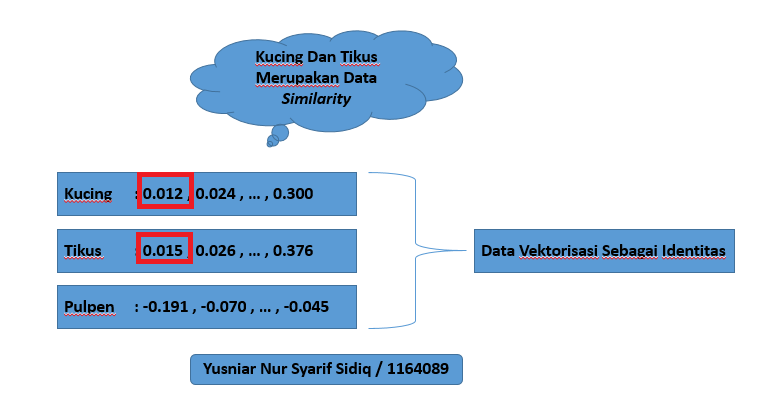
\includegraphics[scale=0.5]{figures/YN/Chapter5/Teori/YNC5-1.png}}
		\caption{Kata-Kata Hasil Vektorisasi}
		\label{YNC5-1}
	\end{figure}

\item Jelaskan mengapa dimensi dari vektor dataset google bisa sampe 300. Dilengkapi dengan ilustrasi atau gambar.
	\subitem Dikarenakan pada setiap dataset didalamnya memiliki identitas masing-masing yang menyebabkan jumlah vektor dataset google bisa sampe 300. Saya akan memberikan sebuah ilustrasi yang saya dapat yaitu bagaimana pembagian dataset pada google. Didalam dataset google tersebut memiliki beberapa objek yaitu spatula, cat, dan dog. Dimana ketiga dataset tersebut akan dilakukan proses perbandingan dataset sehingga diproleh hasil antara cat dan dog yaitu 76\% dikarekan pada dataset cat dan dog memiliki kesamaan data sedangkan untuk hasil perbandingan antara cat dan spatula yaitu 12\%. Mengapa lebih sedikit, dikarenakan data yang dimiliki oleh cat dan spatula tidak memiliki kesamaan data. Hal ini dapat membuktikan setelah dilakukan vektorisasi mesin jadi dapat membedakan mana dataset yang memiliki kesamaan dan mana yang bukan. Mengenai pengertian dan ikustrasi tersebut dapat kita liat kedalam bentuk figure \ref{YNC5-5}

	\begin{figure}[ht]
		\centering{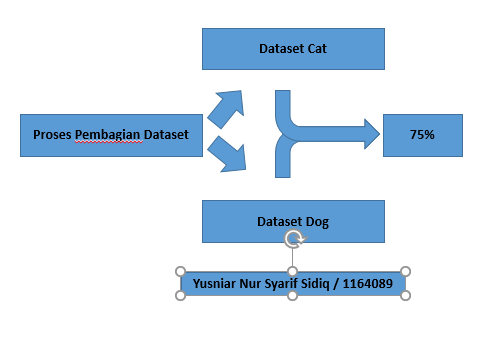
\includegraphics[scale=0.5]{figures/YN/Chapter5/Teori/YNC5-5.png}}
		\caption{Dataset Google}
		\label{YNC5-5}
	\end{figure}

\item Jelaskan konsep vektorisasi untuk kata. Dilengkapi dengan ilustrasi atau gambar.
	\subitem Konsep pada vektorisasi kata yaitu dimana kata tersebut merupakan sebuah hasil pengolahan kata dari sebuah kalimat-kalimat yang telah kita olah. Misalnya saat kita membuka sosial media dan terdapat banyak komentar didalamnya. Ada sebuah kalimat yang mengatakan \" Follow instagram aku yah teman-teman \" , dimana dalam kalimat tersebut memiliki kata kunci instagram dan kata tersebut akan dijadikan data training untuk mesin. Diamana nantinya mesin akan menampilkan kata-kata yang ada kaitannya dengan kata kunci tersebut. Figure \ref{YNC5-3} merupakan sebuah ilustrasi pada vektorisasi kata.

	\begin{figure}[ht]
		\centering{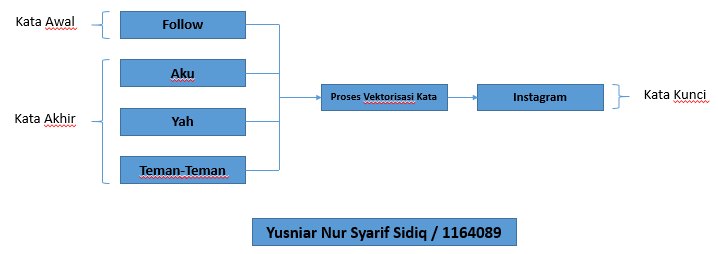
\includegraphics[scale=0.5]{figures/YN/Chapter5/Teori/YNC5-2.png}}
		\caption{Vektorisasi Kata}
		\label{YNC5-2}
	\end{figure}

\item Jelaskan konsep vektorisasi untuk dokumen. Dilengkapi dengan ilustrasi atau gambar.
	\subitem Sebenarnya konsep pada vektorisasi dokumen dan vektorisasi kata itu sama saja, hal yang membedakannya itu hanya proses awalnya. Dimana pada vektorisasi kata akan membaca kalimat per kalimat namun pada vektorisasi dokumen akan membaca keseluruhan kalimat yang terdapat pada sebuah dokumen yang nantinya kalimat-kalimat tersebut akan dipecah menjadia kata per kata. Pada figure \ref{YNC5-3} merupakan contoh ilustrasi sederhana.

	\begin{figure}[ht]
		\centering{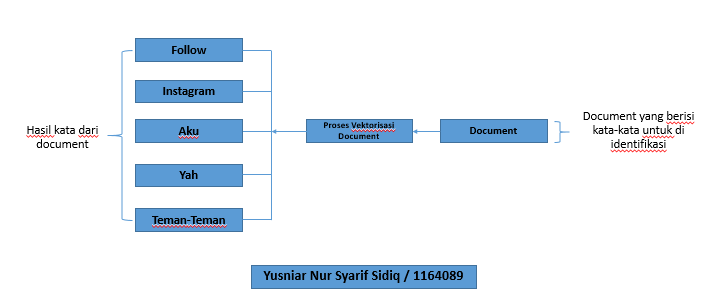
\includegraphics[scale=0.5]{figures/YN/Chapter5/Teori/YNC5-3.png}}
		\caption{Vektorisasi Document}
		\label{YNC5-3}
	\end{figure}

\item Jelaskan apa mean dan standar deviasi. Dilengkapi dengan ilustrasi.
	\subitem Mean merupakan nilai rata-rata dari suatu data. Mean dapat dicari dengan cara membagi jumlah data dengan banyak data sehingga diperoleh lah nilai rata-rata dari suatu data. Sedangkan standar deviasi merupakan sebuah teknik statistik yang digunakan dalam menjelaskan homogenitas kelompok. Contoh sederhananya dimana kita menjumpai dataset yang memiliki 10 data yang berbeda dan 5 atribut yang berbeda. Untuk memperolah nilai mean kita harus menghitung keseluruhan data tersebut lalu hasilnya akan dibagi dengan jumlah datanya. Setelah kita mendapatkan nilai mean maka kita bisa menghitung standar deviasi untuk memperoleh nilai statisknya.

\item Jelaskan apa itu skip-gram. Dilengkapi dengan ilustrasi atau gambar.
	\subitem Skip-gram merupakan sebuah teknik yang digunakan pada area speech processing yang dimana n-gram dibentuk lalu ditambah dengan tindakan skip. Misalkan ada sebuah kalimat yaitu \" I hit the tennis ball \", kita akan membuatnya menjadi skip gram 3 kata maka akan menjadi,
		\begin{itemize}
			\item I hit the
			\item Hit the tennis
			\item The tennis ball
		\end{itemize}
Figure \ref{YNC5-4} merupakan ilustrasi sederhana.
		\begin{figure}[ht]
		\centering{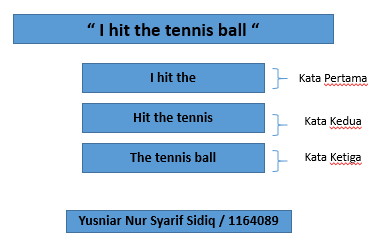
\includegraphics[scale=0.5]{figures/YN/Chapter5/Teori/YNC5-4.png}}
		\caption{Kata-Kata Hasil Vektorisasi}
		\label{YNC5-4}
	\end{figure}

\end{enumerate}

\subsection{Praktek Pemrograman / Yusniar Nur Syarif Sidiq / 1164089}
\begin{enumerate}
\item Cobalah dataset google, dan jelaskan vektor dari kata love, faith, fall, sick, clear, shine, bag, car, wash, motor, cycle dan cobalah untuk melakukan perbandingan similirati dari masing-masing kata tersebut. Jelaskan arti dari outputan similaritas.
	\subitem Dimana output dari source code tersebut merupakan data vektor untuk kata love. Perhatikan figure \ref{YNC5-6}.

		\begin{verbatim}
			gmodel['love']
		\end{verbatim}

		\begin{figure}[ht]
			\centering{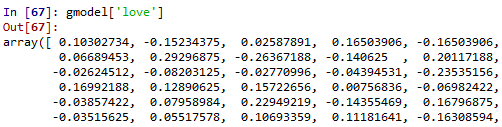
\includegraphics[scale=0.5]{figures/YN/Chapter5/Praktek/YNC5-6.png}}
			\caption{Vektorisasi Kata}
			\label{YNC5-6}
		\end{figure}

Output source code dibawah akan memunculkan data vektor untuk kata faith. Perhatikan figure \ref{YNC5-7}

		\begin{verbatim}
			gmodel['faith']
		\end{verbatim}

		\begin{figure}[ht]
			\centering{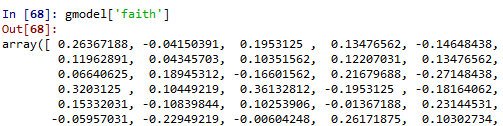
\includegraphics[scale=0.5]{figures/YN/Chapter5/Praktek/YNC5-7.png}}
			\caption{Vektorisasi Kata}
			\label{YNC5-7}
		\end{figure}

Output source code dibawah akan memunculkan data vektor untuk kata fall. Perhatikan figure \ref{YNC5-8}

		\begin{verbatim}
			gmodel['fall']
		\end{verbatim}

		\begin{figure}[ht]
			\centering{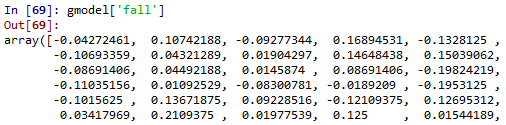
\includegraphics[scale=0.5]{figures/YN/Chapter5/Praktek/YNC5-8.png}}
			\caption{Vektorisasi Kata}
			\label{YNC5-8}
		\end{figure}

Output source code dibawah akan memunculkan data vektor untuk kata sick. Perhatikan figure \ref{YNC5-9}

		\begin{verbatim}
			gmodel['sick']
		\end{verbatim}

		\begin{figure}[ht]
			\centering{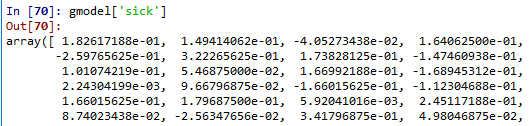
\includegraphics[scale=0.5]{figures/YN/Chapter5/Praktek/YNC5-9.png}}
			\caption{Vektorisasi Kata}
			\label{YNC5-9}
		\end{figure}

Output source code dibawah akan memunculkan data vektor untuk kata clear. Perhatikan figure \ref{YNC5-10}

		\begin{verbatim}
			gmodel['clear']
		\end{verbatim}

		\begin{figure}[ht]
			\centering{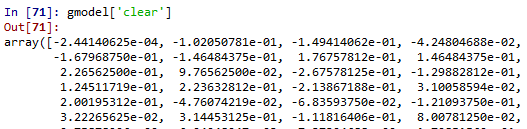
\includegraphics[scale=0.5]{figures/YN/Chapter5/Praktek/YNC5-10.png}}
			\caption{Vektorisasi Kata}
			\label{YNC5-10}
		\end{figure}

Output source code dibawah akan memunculkan data vektor untuk kata shine. Perhatikan figure \ref{YNC5-11}

		\begin{verbatim}
			gmodel['shine']
		\end{verbatim}

		\begin{figure}[ht]
			\centering{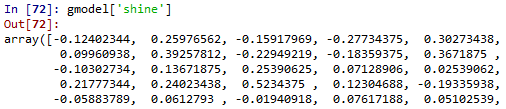
\includegraphics[scale=0.5]{figures/YN/Chapter5/Praktek/YNC5-11.png}}
			\caption{Vektorisasi Kata}
			\label{YNC5-11}
		\end{figure}

Output source code dibawah akan memunculkan data vektor untuk kata bag. Perhatikan figure \ref{YNC5-12}

		\begin{verbatim}
			gmodel['bag']
		\end{verbatim}

		\begin{figure}[ht]
			\centering{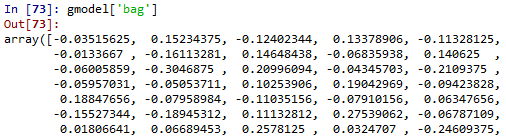
\includegraphics[scale=0.5]{figures/YN/Chapter5/Praktek/YNC5-12.png}}
			\caption{Vektorisasi Kata}
			\label{YNC5-12}
		\end{figure}

Output source code dibawah akan memunculkan data vektor untuk kata car. Perhatikan figure \ref{YNC5-13}

		\begin{verbatim}
			gmodel['car']
		\end{verbatim}

		\begin{figure}[ht]
			\centering{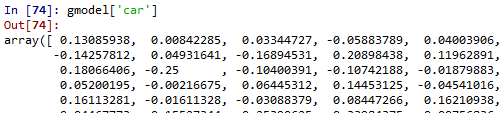
\includegraphics[scale=0.5]{figures/YN/Chapter5/Praktek/YNC5-13.png}}
			\caption{Vektorisasi Kata}
			\label{YNC5-13}
		\end{figure}

Output source code dibawah akan memunculkan data vektor untuk kata wash. Perhatikan figure \ref{YNC5-14}

		\begin{verbatim}
			gmodel['wash']
		\end{verbatim}

		\begin{figure}[ht]
			\centering{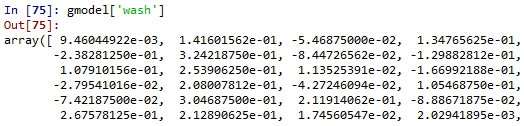
\includegraphics[scale=0.5]{figures/YN/Chapter5/Praktek/YNC5-14.png}}
			\caption{Vektorisasi Kata}
			\label{YNC5-14}
		\end{figure}
Output source code dibawah akan memunculkan data vektor untuk kata motor. Perhatikan figure \ref{YNC5-15}

		\begin{verbatim}
			gmodel['motor']
		\end{verbatim}

		\begin{figure}[ht]
			\centering{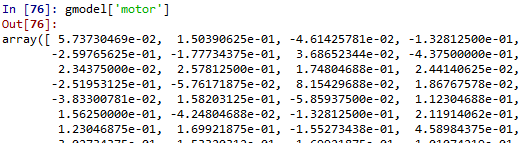
\includegraphics[scale=0.5]{figures/YN/Chapter5/Praktek/YNC5-15.png}}
			\caption{Vektorisasi Kata}
			\label{YNC5-15}
		\end{figure}

Output source code dibawah akan memunculkan data vektor untuk kata cycle. Perhatikan figure \ref{YNC5-16}

		\begin{verbatim}
			gmodel['cycle']
		\end{verbatim}

		\begin{figure}[ht]
			\centering{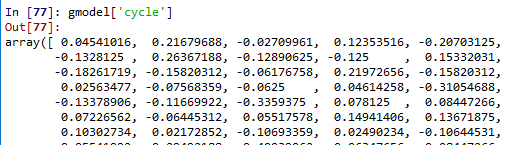
\includegraphics[scale=0.5]{figures/YN/Chapter5/Praktek/YNC5-16.png}}
			\caption{Vektorisasi Kata}
			\label{YNC5-16}
		\end{figure}

	\subitem Pada source code dibawah menunjukkan hasil score perbandingan kata apakah kata cycle dan motor memiliki ke samaan atau tidak, perhatikan figure \ref{YNC5-17}

		\begin{verbatim}
			gmodel.similarity('cycle','motor')
		\end{verbatim}

		\begin{figure}[ht]
			\centering{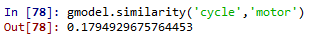
\includegraphics[scale=0.5]{figures/YN/Chapter5/Praktek/YNC5-17.png}}
			\caption{Perbandingan Kata}
			\label{YNC5-17}
		\end{figure}

Pada source code dibawah menunjukkan hasil score perbandingan kata apakah kata car dan wash memiliki ke samaan atau tidak, perhatikan figure \ref{YNC5-18}

		\begin{verbatim}
			gmodel.similarity('car','wash')
		\end{verbatim}

		\begin{figure}[ht]
			\centering{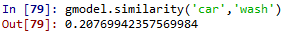
\includegraphics[scale=0.5]{figures/YN/Chapter5/Praktek/YNC5-18.png}}
			\caption{Perbandingan Kata}
			\label{YNC5-18}
		\end{figure}

Pada source code dibawah menunjukkan hasil score perbandingan kata apakah kata bag dan shine memiliki ke samaan atau tidak, perhatikan figure \ref{YNC5-19}

		\begin{verbatim}
			gmodel.similarity('bag','shine')
		\end{verbatim}

		\begin{figure}[ht]
			\centering{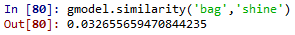
\includegraphics[scale=0.5]{figures/YN/Chapter5/Praktek/YNC5-19.png}}
			\caption{Perbandingan Kata}
			\label{YNC5-19}
		\end{figure}

Pada source code dibawah menunjukkan hasil score perbandingan kata apakah kata clear dan sick memiliki ke samaan atau tidak, perhatikan figure \ref{YNC5-20}

		\begin{verbatim}
			gmodel.similarity('clear','sick')
		\end{verbatim}

		\begin{figure}[ht]
			\centering{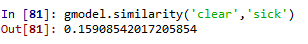
\includegraphics[scale=0.5]{figures/YN/Chapter5/Praktek/YNC5-20.png}}
			\caption{Perbandingan Kata}
			\label{YNC5-20}
		\end{figure}

Pada source code dibawah menunjukkan hasil score perbandingan kata apakah kata fall dan faith memiliki ke samaan atau tidak, perhatikan figure \ref{YNC5-21}

		\begin{verbatim}
			gmodel.similarity('fall','faith')
		\end{verbatim}

		\begin{figure}[ht]
			\centering{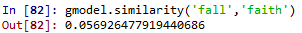
\includegraphics[scale=0.5]{figures/YN/Chapter5/Praktek/YNC5-21.png}}
			\caption{Perbandingan Kata}
			\label{YNC5-21}
		\end{figure}

\item Jelaskan dengan kata dan ilustrasi fungsi dari extact\_words dan PermuteSentences.
		
		\begin{verbatim}
		import re
		def extract_words(sent):
    			sent = sent.lower()
   		 	sent = re.sub(r'<[^>]+>', ' ', sent) 
    			sent = re.sub(r'(\w)\'(\w)', ' ', sent) 
    			sent = re.sub(r'\W', ' ', sent) 
    			sent = re.sub(r'\s+', ' ', sent) 
    		return sent.split()
		\end{verbatim}
	\subitem Dimana source code tersebut akan membersihkan tag-tag yang tidak perlu dan mengubahnya ke dalam bentuk array list perkata menggunakan split.

		\begin{verbatim}
		import random
		class PermuteSentences(object):
    			def __init__(self, sents):
        				self.sents = sents
        
    			def __iter__(self):
        		shuffled = list(self.sents)
        		random.shuffle(shuffled)
        			for sent in shuffled:
            		yield sent
		\end{verbatim}
	\subitem Dimana source code diatas berfungsi untuk melakukan pengacakan data supaya memperoleh data yang teratur.

\end{enumerate}

\section{Imron Sumadireja / 1164076}
\subsection{Teori}
\begin{enumerate}
\item Jelaskan kenapa kata-kata harus dilakukan vektorisasi. Dilengkapi dengan ilustrasi \par
Karena untuk mengetahui presentase kata yang sering muncul dalam setiap kalimatnya, yang berguna untuk menetukan kata kunci, serta untuk memberikan kemudahan bagi mesin untuk mempelajari kata yang bentuk aslinya serupa namun tak sama seperti bebek dan ayam. Selain itu fungsi dari vektorisasi kata ini untuk membaca setiap kata-katanya dengan merubah kata menjadi sebuah angka atau identitas itu sendiri \ref{vek1}.
		\begin{figure}[ht]
		\centerline{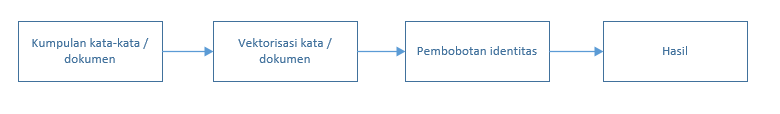
\includegraphics[width=0.5\textwidth]{figures/im/vek1.png}}
		\caption{Ilustrasi Vektorisasi Kata.}
		\label{vek1}
		\end{figure}

\item Jelaskan mengapa dimensi dari vektor dataset google bisa sampai 300. Dilengkapi dengan ilustrasi \par
Karena pada masing-masing objek itu memiliki identitas tersendiri, contoh sederhananya. Pada dataset google ini memiliki 3 buah objek diantaranya, cat, dog, dan spatula. Lalu dari masing-masing objek itu dibandingkan datasetnya antara cat dan dog lalu cat dan spatula. Hasil yang didapatkan untuk cat dan dog itu sekitar 76\% sedangkan untuk cat dan spatula itu memiliki presentase 12\% itu artinya bahwa mesin dapat membedakan objek yang hampir serupa namun tak sama. Untuk ilustrasi sederhananya bisa dilihat pada gambar \ref{vek2}.
		\begin{figure}[ht]
		\centerline{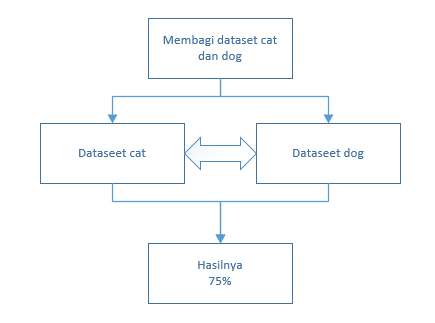
\includegraphics[width=0.5\textwidth]{figures/im/vek2.png}}
		\caption{Ilustrasi Vektorisasi Dataset Google.}
		\label{vek2}
		\end{figure}

\item Jelaskan konsep vektorisasi untuk kata. Dilengkapi dengan ilustrasi \par
Konsep untuk vektorisasi kata ini sama halnya dengan kita input suatu kata pada mesin pencari. Lalu hasilnya akan mengeluarkan berupa referensi mengenai kata tersebut. Jadi data kata tersebut didapatkan dari hasil pengolahan pada kalimat-kalimat sebelumnya yang telah diolah. Contoh sederhananya pada kalimat berikut ( Please subscribe my channel thank you guys ), pada kalimat tersebut terdapat konteks yakni channel, kata tersebut akan dijadikan data latih untuk mesin. Jadi ketika kita inputkan kata channel, maka mesin akan menampilkan keterkaitannya dengan kata tersebut. Ilustrasinya bisa dilihat pada gambar berikut \ref{vek3}.
		\begin{figure}[ht]
		\centerline{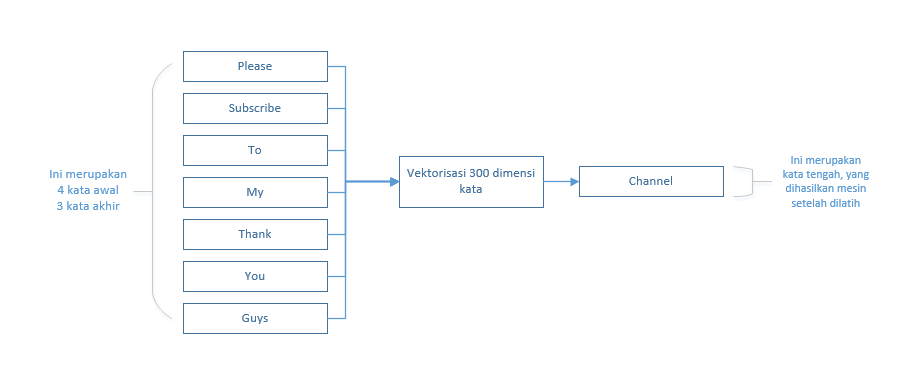
\includegraphics[width=0.5\textwidth]{figures/im/vek3.png}}
		\caption{Ilustrasi Vektorisasi Kata.}
		\label{vek3}
		\end{figure}

\item Jelaskan konesep vektorisasai untuk dokumen. Dilengkapi dengan ilustrasi \par
Sama halnya dengan vektorisasi kata, yang membedakan hanya pada proses awalnya. Untuk vektorisasi dokumen ini, mesin akan membaca semua kalimat yang terdapat pada dokumen tersebut, lalu kalimat yang terdapat pada dokumen akan di pecah menjadi kata-kata. Untuk ilustrasinya dapat dilihat pada gambar berikut \ref{vek4}.
		\begin{figure}[ht]
		\centerline{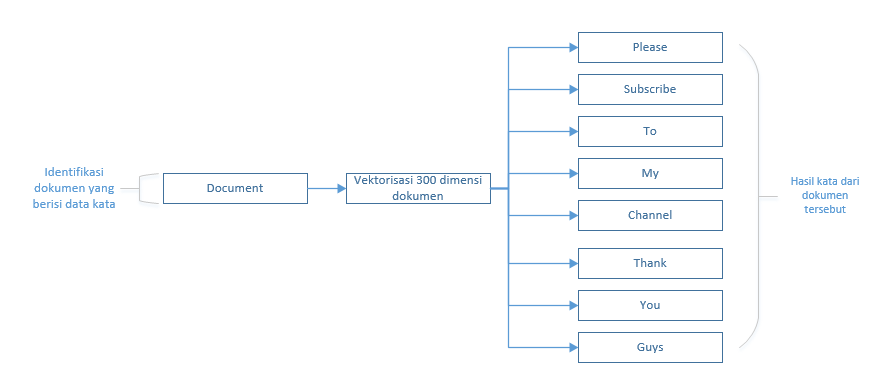
\includegraphics[width=0.5\textwidth]{figures/im/vek4.png}}
		\caption{Ilustrasi Vektorisasi Dokumen.}
		\label{vek4}
		\end{figure}

\item Jelaskan apa mean dan standar deviasi. \par
Mean merupakan nilai rata-rata. Untuk mendapatkan mean ini kita tinggal menjumlahkan data yang tersedia lalu dibagi dengan banyaknya data tersebut. Sedangkan standar deviasi adalah nilai statistik yang digunakan untuk menentukan bagaimana sebaran data dalam sampel, dan seberapa dekat titik data individu dengan rata-rata nilai sampel.

\item Jelaskan apa itu skip-gram. Dilengkapi dengan ilustrasi \par
Skip-gram sama halnya dengan vektorisasi kata, namun untuk skip-gram ia dibalik prosesnya. Yang sebelumnya dari kalimat lalu di olah untuk menemukan salah satu kata, kali ini dari keyword tersebut akan diolah menjadi suatu kalimat yang memiliki keterkaitannya dengan keyword tersebut. Ilustrasinya bisa dilihat pada gambar berikut \ref{vek5}.
		\begin{figure}[ht]
		\centerline{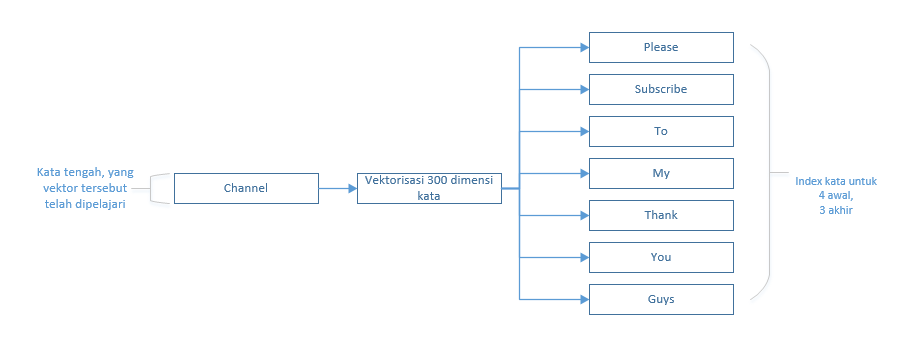
\includegraphics[width=0.5\textwidth]{figures/im/vek5.png}}
		\caption{Ilustrasi Skip-Gram.}
		\label{vek6}
		\end{figure}

\end{enumerate}

\subsection{Praktikum / Imron Sumadireja / 1164076}
\begin{enumerate}
\item Cobalah dataset google, dan jelaskan vektor dari kata love, faith, fall, sick, clear, shine, bag, car, wash, motor, cycle dan cobalah untuk melakukan perbandingan similirati dari masing-masing kata tersebut \par
\begin{verbatim}
import gensim, logging
logging.basicConfig(format='%(asctime)s : %(levelname)s : %(message)s', level=logging.INFO)
gmodel = gensim.models.KeyedVectors.load_word2vec_format('F:/Imron/Kuliah/Semester 6/../GoogleNews-vectors-negative300.bin', binary=True, limit=500000)
\end{verbatim}
Hasil keluaran pada gambar \ref{sim1} untuk keluaran ke 99 itu untuk import library gensim. Gensim itu sendiri berguna untuk melakukan pemodelan dengan dataset atau topik yang telah ditentukan. Untuk keluaran 100 logging itu library opsional karena logging hanya untuk menampilkan berupa log untuk setiap code yang dijalankan. Dan keluaran 101 itu hasil load data dari file vektor google itu, disini saya menggunakan limit karena kondisi laptop yang tidak mempuni untuk melakukan running data sebesar 3 juta file, jadi saya batasi hanya melakukan running 500 ribu data saja.
		\begin{figure}[ht]
		\centerline{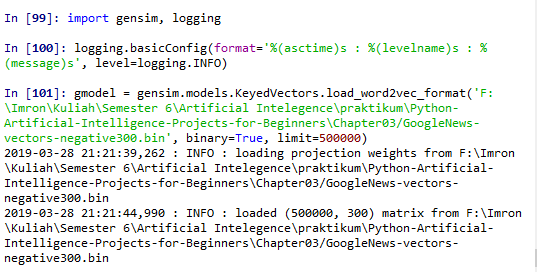
\includegraphics[width=0.5\textwidth]{figures/im/sim1.png}}
		\caption{Hasil import gensim dan logging.}
		\label{sim1}
		\end{figure}

\begin{verbatim}
gmodel['love']
\end{verbatim}
Keluaran pada gambar \ref{sim2} ini untuk menampilkan data hasil vektorisasi data dari kata love, hasil tersebut berjumlah kurang lebih 300 data. Untuk kata faith, fall, sick, clear, dan lain-lain itu sama saja untuk menampilkan hasil vektorisasi dari setiap katanya. Selanjutnya akan dibandingkan setiap katanya untuk menentukan presentase kemiripan pada setiap kata tersebut.
		\begin{figure}[ht]
		\centerline{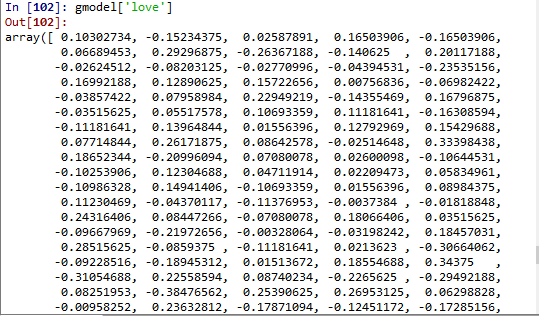
\includegraphics[width=0.5\textwidth]{figures/im/sim2.png}}
		\caption{Data vektor dari kata love.}
		\label{sim2}
		\end{figure}

\begin{verbatim}
gmodel.similarity('love','faith')
\end{verbatim}
Hasil keluaran pada gambar \ref{sim3} merupakan presentase dari perbandingan kata love dan faith dengan hasil 37\%. Hasil tersebut didapatkan dengan 37\% karena mesin dapat membaca bahwa kata love dengan faith ini hampir memiliki arti yang sama.
		\begin{figure}[ht]
		\centerline{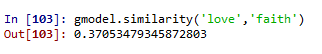
\includegraphics[width=0.5\textwidth]{figures/im/sim3.png}}
		\caption{Hasil similaritas.}
		\label{sim3}
		\end{figure}

\begin{verbatim}
gmodel.similarity('fall','sick')
\end{verbatim}
Hasil keluaran pada gambar \ref{sim4} adalah hasil presentase dari perbandingan antara kata fall dan sick dengan hasil 8\%. Hasil tersebut tidak terlalu baik, karena mesin menentukan bahwa kata fall dengan sick itu tidak serupa karena memiliki presentase yang kecil.
		\begin{figure}[ht]
		\centerline{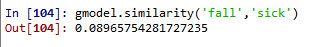
\includegraphics[width=0.5\textwidth]{figures/im/sim4.png}}
		\caption{Hasil similaritas.}
		\label{sim4}
		\end{figure}

\begin{verbatim}
gmodel.similarity('clear','shine')
\end{verbatim}
Hasil keluaran pada gambar \ref{sim5} merupakan hasil presentase dari perbandingan antara kata clear dengan shine dengan hasil presentase 11\%. Presentase tersebut dapat memberikan kita gambaran bahwa mesin dapat menentukan bahwa kata clear dan shine itu berbeda.
		\begin{figure}[ht]
		\centerline{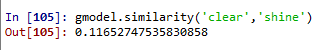
\includegraphics[width=0.5\textwidth]{figures/im/sim5.png}}
		\caption{Hasil similaritas.}
		\label{sim5}
		\end{figure}

\begin{verbatim}
gmodel.similarity('bag','wash')
\end{verbatim}
Hasil keluaran pada gambar \ref{sim6} adalah hasil presentase dari perbandingan kata bag dengan wash dan hasil presentasenya 18\%. Presentase tersebut cukup bagus karena mesin dapat membedakan kata antara bag dan wash.
		\begin{figure}[ht]
		\centerline{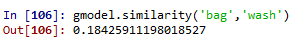
\includegraphics[width=0.5\textwidth]{figures/im/sim6.png}}
		\caption{Hasil similaritas.}
		\label{sim6}
		\end{figure}

\begin{verbatim}
gmodel.similarity('car','motor')
\end{verbatim}
Hasil keluaran pada gambar \ref{sim7} merupakan hasil dari perbandingan kata car dengan motor dan hasil presentasenya 48\%. Ini terbilang bagus dan bisa dikatakan mirip karena mesin dapat menentukan presentase yang cukup baik.
		\begin{figure}[ht]
		\centerline{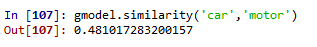
\includegraphics[width=0.5\textwidth]{figures/im/sim7.png}}
		\caption{Hasil similaritas.}
		\label{sim7}
		\end{figure}

\item Jelaskan dengan kata dan ilustrasi fungsi dari extract words dan PermuteSentences
\begin{verbatim}
import re
def extract_words(sent):
    sent = sent.lower()
    sent = re.sub(r'<[^>]+>', ' ', sent) #hapus tag html
    sent = re.sub(r'(\w)\'(\w)', ' ', sent) #hapus petik satu
    sent = re.sub(r'\W', ' ', sent) #hapus tanda baca
    sent = re.sub(r'\s+', ' ', sent) #hapus spasi yang berurutan
    return sent.split()
\end{verbatim}
Code tersebut berguna untuk menghapus tag-tag html yang tidak diperlukan pada dokumen yang telah dilakukan pelatihan dan vektorisasi, hasilnya pun tidak mengeluarkna apa-apa, hanya pemberitahuan bahwa code tersebut telah berhasil dijalankan. Dan code tersebut akan merubah kalimat yang didalamnya menjadi list kata-kata dalam bentuk array dengan menggunakan split.

\begin{verbatim}
import random
class PermuteSentences(object):
    def __init__(self, sents):
        self.sents = sents
        
    def __iter__(self):
        shuffled = list(self.sents)
        random.shuffle(shuffled)
        for sent in shuffled:
            yield sent
\end{verbatim}
Code tersebut untuk melakukan pengacakan data agar data tersebut dapat menghasilkan hasil yang mempuni. Code tersebut bisa digunakan atau tidak, tetapi alangkah baiknya untuk digunakan agar hasil akhir yang didapatkan bisa prima.

\item Jelaskan fungsi dari librari gensim TaggedDocument dan Doc2Vec disertai praktek pemakaiannya
\begin{verbatim}
from gensim.models.doc2vec import TaggedDocument
from gensim.models import Doc2Vec
\end{verbatim}
Fungsi dari doc2vec itu sendiri ialah untuk membandingkan data yang terdapat pada dokumen yang lainnya, apakah kata-kata didalamnya ada yang sama atau tidak. Lalu untuk tagged document itu memasukan kata-kata pada setiap dokumennya untuk di vektorisasi.
\end{enumerate}